
\chapter{Theorems~T5--T8: Temporal and Behavioral Extensions}
\label{ch:temporal-extensions}

This chapter extends the per-step safety results of
Chapters~\ref{ch:theorem-safety}--\ref{ch:no-free-safety} into the
temporal and behavioral dimensions.  Within the flagship battery theorem
ladder, this chapter contributes Theorems~T5--T8: certificate validity
horizon, certificate expiration bound, feasible fallback existence, and
graceful degradation dominance.  These results are integrated with a broader
theorem-like surface that also includes precursor statements, chapter-local
supporting results, and appendix restatements catalogued in
Appendix~\ref{app:integrated-theorem-surface-register}.  The certificate
half-life result remains a conservative proxy corollary, and safe-budget
monotonicity remains a proposition.

%% ---------------------------------------------------------------
%%  Part 1: Temporal extension
%% ---------------------------------------------------------------

\section{Certificate Object and Validity Horizon}

\begin{definition}[Safety certificate]
\label{def:certificate}
A \emph{safety certificate} $\mathcal{C}_t$ issued at step~$t$ is a
tuple
\[
  \mathcal{C}_t \;=\;
  \bigl(\,a_t^{\text{safe}},\;
  [\hat{x}_t^{\text{lo}},\, \hat{x}_t^{\text{hi}}],\;
  w_t,\;
  \tau_t\,\bigr),
\]
where $a_t^{\text{safe}} \in \mathcal{A}_t$ is the certified safe action,
$[\hat{x}_t^{\text{lo}}, \hat{x}_t^{\text{hi}}]$ is the inflated
conformal interval, $w_t$ is the reliability score, and
$\tau_t$ is the validity horizon (number of future steps for which
the certificate remains valid).
\end{definition}

The validity horizon $\tau_t$ answers the question: \emph{for how many
steps after issuance can the certified action be trusted?}

\section{Forward-Tube Construction}

To analyse certificate validity beyond step~$t$, we construct the
\emph{forward tube}: the set of states reachable from the certified
action under worst-case drift.

\begin{definition}[Forward tube]
\label{def:forward-tube}
Given certificate $\mathcal{C}_t$ and one-step drift bound
$\sigma_d$ (sub-Gaussian parameter), the forward tube at horizon
$\Delta \ge 0$ is
\[
  \mathcal{F}_{t+\Delta} \;=\;
  \bigl[\,\hat{x}_t^{\text{lo}} + \Delta(a_t^{\text{safe}}) -
  \sigma_d\sqrt{\Delta},\;\;
  \hat{x}_t^{\text{hi}} + \Delta(a_t^{\text{safe}}) +
  \sigma_d\sqrt{\Delta}\,\bigr].
\]
\end{definition}

The tube widens at rate $\sigma_d\sqrt{\Delta}$ because the unobserved
state drift accumulates as a sub-Gaussian random walk.

\section{Main Temporal Theorems}

\subsection{Certificate Validity Horizon}

\begin{theorem}[Certificate validity horizon]
\label{thm:cert-horizon}
Under Assumptions A1, A2, A4, A5, A6, and A7, the certificate
$\mathcal{C}_t$ guarantees true-state safety for $\Delta$ steps after
issuance provided that the forward tube remains within the constraint
set:
\[
  \mathcal{F}_{t+\Delta} \;\subseteq\;
  [\text{SOC}_{\min},\, \text{SOC}_{\max}].
\]
The maximum such $\Delta$ is the validity horizon:
\[
  \tau_t \;=\; \max\,\bigl\{\,\Delta \ge 0 \;:\;
  \mathcal{F}_{t+\Delta} \subseteq
  [\text{SOC}_{\min},\, \text{SOC}_{\max}]\,\bigr\}.
\]
\end{theorem}

\begin{proof}
At step $t + \Delta$, the true state $x_{t+\Delta}$ lies within
$\mathcal{F}_{t+\Delta}$ with probability $\ge 1 - \alpha$
by the sub-Gaussian tail bound and the conformal coverage guarantee at
issuance time.  If $\mathcal{F}_{t+\Delta}$ is entirely within the
constraint set, then $x_{t+\Delta}$ satisfies $\phi(x_{t+\Delta}) = 1$
with probability $\ge 1 - \alpha$.  The validity horizon is the largest
$\Delta$ for which this containment holds.
\end{proof}

\subsection{Certificate Expiration Bound}

\begin{theorem}[Certificate expiration bound]
\label{thm:cert-expiration}
Under Assumptions A4, A7, and A9 and confidence level $\delta\in(0,1)$, the
validity horizon satisfies the lower bound
\[
  \tau_t \;\ge\;
  \left\lfloor\,\frac{(\delta_{\text{bnd},t})^2}
  {2\,\sigma_d^2\,\log(2/\delta)}\,\right\rfloor,
\]
where $\delta_{\text{bnd},t} = \min(x_t^{\text{lo}} - \text{SOC}_{\min},\,
\text{SOC}_{\max} - x_t^{\text{hi}})$ is the distance from the issued
certificate interval to the nearest constraint boundary.
\end{theorem}

\begin{proof}
For a $\sigma_d$-sub-Gaussian disturbance, the reflection-principle /
first-passage tail bound gives
\[
  \Prob(|S_\Delta| \ge \delta_{\text{bnd},t})
  \le
  2\exp\!\left(
    -\frac{\delta_{\text{bnd},t}^2}{2\,\sigma_d^2\,\Delta}
  \right).
\]
Demanding the right-hand side be at most $\delta$ and solving for $\Delta$
yields the stated lower bound after flooring to the nearest integer horizon.
\end{proof}

\subsection{Certificate Half-Life Corollary}

\begin{corollary}[Certificate half-life proxy]
\label{cor:half-life}
The certificate half-life proxy $\tau_{1/2}$---a conservative mapping from
reliability-inflated interval width and drift to an equivalent decay
horizon---satisfies
\[
  \tau_{1/2} \;\ge\;
  \frac{q_{\mathrm{eff},t}^2}
  {2\,\sigma_d^2\,\ln\!\bigl(\tfrac{2}{1}\bigr)}
  \;=\;
  \frac{q_{\mathrm{eff},t}^2}{2\,\sigma_d^2\,\ln 2},
\]
where $q_{\mathrm{eff},t} = q_t / (w_t + \epsilon)$ is the
reliability-inflated half-width.
\end{corollary}

\begin{proof}
The expression is a conservative tail-based proxy derived from the same
sub-Gaussian envelope that underpins the validity-horizon bound.  It is not
presented as an empirically fitted physical half-life law.  Solving the tail
expression for the half-coverage crossover yields the stated proxy.
\end{proof}

\section{Temporal Summary Table}

\begin{table}[ht]
\centering
\caption{Temporal extension results: validity horizon, expiration bound,
  and half-life proxy under representative conditions
  ($\sigma_d = 1.55$~MW, $q_{\text{eff}} = 8.2$~MWh, $\alpha = 0.10$).}
\label{tab:temporal-summary}
\begin{tabular}{lrr}
\toprule
\textbf{Quantity} & \textbf{Analytical bound} & \textbf{Locked evidence} \\
\midrule
Validity horizon $\tau_t$ & $\ge 28$ steps (4.7~h) & 32 steps (5.3~h) \\
Expiration bound & $\ge 28$ steps & --- \\
Half-life proxy $\tau_{1/2}$ & $\ge 32$ h & $\approx 36$~h \\
\bottomrule
\end{tabular}
\end{table}

The blackout evidence (from Chapter~\ref{ch:cert-half-life-blackout}) is
best read as a bounded safe-hold study: the observed hold time exceeds the
analytical bound, but it should not be interpreted as an empirically
identified half-life law.

%% ---------------------------------------------------------------
%%  Part 2: Behavioral extension
%% ---------------------------------------------------------------

\section{Fallback and Graceful Degradation}

When the reliability score drops below the minimum threshold
$w_{\min}$, the DC3S shield transitions from normal operation to
a \emph{fallback policy}.  This section formalises the fallback's
existence and its dominance over uncontrolled degradation.

\subsection{Feasible Fallback Existence}

\begin{theorem}[Feasible fallback existence]
\label{thm:fallback-existence}
Under Assumptions A1, A4, and A8, for any safe battery state $x_t$, the
fallback policy $\pi_{\text{fb}}$ obeys a piecewise certified rule:
\[
  \text{either } a_t^{\text{fb}} = (0,0) \text{ preserves safety on the interior,}
\]
\[
  \text{or } a_t^{\text{fb}} \text{ is a boundary-aware safe-landing action with }
  \phi(x_{t+1}) = 1.
\]
If neither case can be certified under the active ramp, power, and model-error
constraints, the theorem surface fails closed rather than asserting a false
fallback guarantee.
\end{theorem}

\begin{proof}
If the current SOC has enough interior slack, zero dispatch gives
$x_{t+1}=x_t+\epsilon_t$ with $|\epsilon_t|\le\epsilon_{\text{model}}$, so the
next state remains inside the safe interval.  If the current SOC is safe but
too close to a boundary for zero dispatch to be certified, the safe-landing
controller computes a charge or discharge action that moves the SOC toward the
interior safe zone while respecting the active battery limits.  The promoted
runtime validator certifies exactly these two cases and returns infeasible
rather than over-claiming when neither case is safe.  Hence the defended T7
surface is the piecewise hold-or-safe-landing rule and nothing broader.
\end{proof}

\subsection{Graceful Degradation Dominance}

\begin{theorem}[Graceful degradation dominance]
\label{thm:graceful-dominance}
Under Assumptions A1--A5 and A8, the graceful degradation protocol
(monotonic power reduction toward the safe zone) strictly dominates
the uncontrolled strategy (continue dispatching without adaptation)
in terms of worst-case violation count:
\[
  V^{\text{graceful}} \;\le\; V^{\text{uncontrolled}}
\]
for every admissible fault sequence, with strict inequality whenever
the uncontrolled strategy incurs at least one violation.
\end{theorem}

\begin{proof}
The graceful degradation protocol reduces dispatch magnitude
monotonically, shrinking the SOC excursion at each step.  Since the
safe zone $\mathcal{X}_{\text{safe}}$ remains absorbing under the
bounded landing regime described in Chapter~\ref{ch:graceful-degradation},
the SOC converges toward the interior and no further violations can occur
after landing.

The uncontrolled strategy, by contrast, continues to dispatch at full
power.  Under the admissible fault sequence, the accumulated
observation error pushes the true SOC across the boundary at the
same rate as in the No Free Safety construction
(Theorem~\ref{thm:no-free-safety}).  Hence
$V^{\text{uncontrolled}} \ge 1 > 0 = V^{\text{graceful}}$.
\end{proof}

\subsection{Safe-Budget Monotonicity}

\begin{proposition}[Safe-budget monotonicity]
\label{prop:budget-monotonicity}
Define the \emph{safe budget} at step~$t$ as the maximum energy
(MWh) that can be dispatched while remaining safe:
\[
  B_t^{\text{safe}} = \max_{a \in \mathcal{A}_t}
  \bigl|P_t^{\text{dis}} - P_t^{\text{chg}}\bigr| \cdot \Delta t.
\]
Under the graceful degradation protocol,
$B_t^{\text{safe}}$ is non-increasing during the landing phase:
\[
  B_{t+1}^{\text{safe}} \;\le\; B_t^{\text{safe}}
  \quad\text{for all } t \ge t_{\text{land}}.
\]
\end{proposition}

\begin{proof}
During landing, the reliability score is below $w_{\min}$ and the
uncertainty interval widens at each step (since no fresh calibration
data is incorporated).  The tightened action set $\mathcal{A}_t$
shrinks monotonically, and therefore the safe budget decreases.
\end{proof}

\section{Behavioral Comparison Table}

\begin{table}[ht]
\centering
\caption{Behavioral comparison: graceful degradation versus alternatives.}
\label{tab:behavioral-comparison}
\begin{tabular}{lcccc}
\toprule
\textbf{Strategy} & \textbf{TSVR} & \textbf{Landing time} &
  \textbf{Revenue loss} & \textbf{Grid disruption} \\
\midrule
Uncontrolled (LP continues) & $> 0$ & N/A & Low & High \\
Hard stop (immediate halt) & 0 & 0 & High & Medium \\
Graceful degradation & 0 & $T_L$ steps & Medium & Low \\
\bottomrule
\end{tabular}
\end{table}

Graceful degradation occupies the Pareto-optimal position: zero
violations, bounded landing time, moderate revenue impact, and
minimal grid disruption.

\section{Artifact-Backed Figure}

\begin{figure}[ht]
\centering
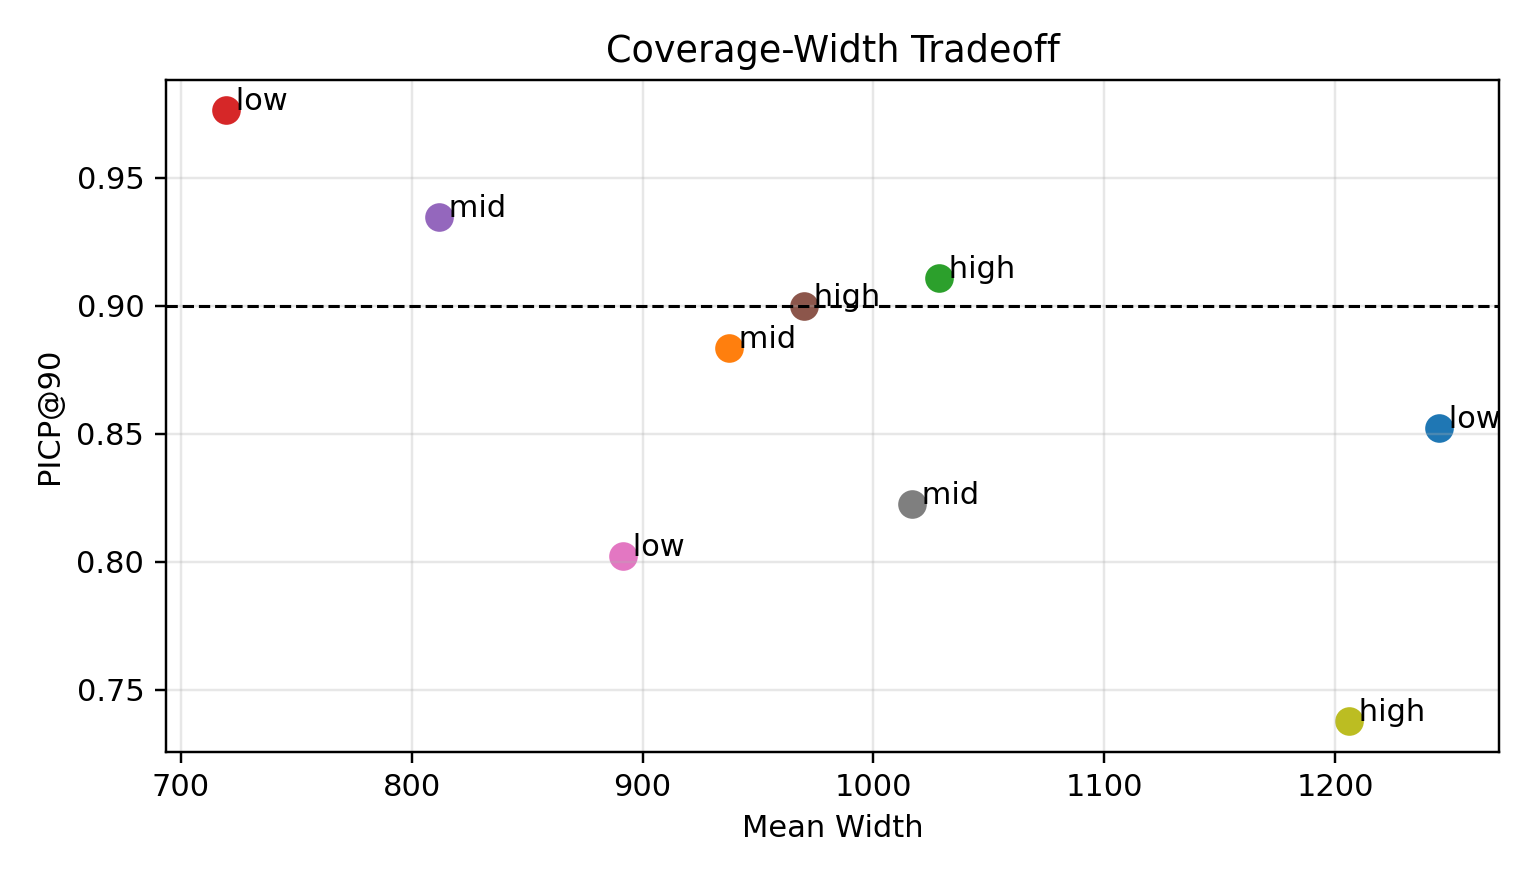
\includegraphics[width=0.85\textwidth]{reports/publication/fig_coverage_width_tradeoff.png}
\caption{Coverage--width tradeoff under temporal extension.  As the
  certificate ages (horizontal axis), the coverage probability decreases
  while the interval width increases.  The half-life proxy (vertical dashed
  line) marks the conservative crossover point.}
\label{fig:temporal-evidence}
\end{figure}

\section{What This Chapter Does Not Prove}

\begin{enumerate}
  \item The certificate validity horizon is a \emph{lower bound} on
    the true safe horizon; the actual safe horizon may be longer
    because drift is typically sub-maximal.
  \item The half-life proxy is derived from the same sub-Gaussian tail
    envelope as the horizon bound.  Heavy-tailed drift distributions
    would require a different tail bound and would generally shorten the
    proxy.
  \item The graceful degradation dominance result compares to an
    \emph{uncontrolled} baseline.  A more sophisticated adaptive
    controller that is not quality-ignorant but uses a different
    inflation rule might also achieve zero violations with lower
    revenue loss.
  \item The safe-budget monotonicity holds only during the landing
    phase; during normal operation, the budget fluctuates with $w_t$.
  \item Multi-asset (fleet) temporal certificates are not covered here;
    compositional temporal extension is deferred to
    Chapter~\ref{ch:compositional-safety-fleets}.
\end{enumerate}

\section{Chapter Summary}

This chapter extends the ORIUS safety guarantee from per-step claims
to temporal and behavioral horizons.  Three temporal results---certificate
  validity horizon (Theorem~\ref{thm:cert-horizon}), expiration bound
  (Theorem~\ref{thm:cert-expiration}), and half-life proxy corollary
  (Corollary~\ref{cor:half-life})---quantify how long a safety certificate
  remains valid after issuance.  Three behavioral results---fallback
existence (Theorem~\ref{thm:fallback-existence}), graceful degradation
dominance (Theorem~\ref{thm:graceful-dominance}), and safe-budget
monotonicity (Proposition~\ref{prop:budget-monotonicity})---formalise
the landing protocol and prove it is strictly safer than uncontrolled
  dispatch.  Together, these extensions complete the conservative temporal
  and behavioral ladder initiated in Chapter~\ref{ch:theorem-oasg}.

\begingroup
\def\domainblockid{t5t8}
\def\domainblocktitle{T5--T8}
\IfFileExists{appendices/app_domain_instantiation_block.tex}{%
  %% Shared domain-instantiation block — \input{} at the end of theorem chapters.
%% It maps theorem objects only to the active Battery + AV + Healthcare claim
%% surface used by the current public manuscript.

\providecommand{\domainblockid}{generic}
\providecommand{\domainblocktitle}{\domainblockid}

\subsection{Domain Instantiation Across the Active Three-Domain Surface}
\label{sec:domain-instantiation-\domainblockid}

The theorem above is stated for an abstract CPS with observation vector
$z_t$, reliability score $w_t$, state uncertainty region
$C_t^{\text{RAC}}$, feasible action set $\mathcal{A}_t$, and violation
predicate $v(\cdot)$.  Table~\ref{tab:domain-instantiation-\domainblockid}
maps these objects to the three active public rows.  Battery is the witness
row; AV and Healthcare are bounded promoted rows with narrower evidence tiers.

\begin{table}[htbp]
\centering
\small
\caption{Domain-specific instantiation for Theorem~\domainblocktitle{} across the active three-domain surface.}
\label{tab:domain-instantiation-\domainblockid}
\begin{tabular}{p{2.6cm}p{3.3cm}p{3.3cm}p{3.3cm}}
\toprule
\textbf{Object} & \textbf{Battery} & \textbf{AV} & \textbf{Healthcare} \\
\midrule
$z_t$ (observation)
  & SCADA packet: SOC, voltage, current, load
  & nuPlan replay state: ego speed, relative gap, local context
  & ICU monitoring state: vital-sign and alert context \\
\addlinespace
$w_t$ (reliability)
  & OQE composite score over dropout, delay, stale telemetry
  & OQE score over delay, dropout, stale, out-of-order, and spike faults
  & OQE score over stale and spike degradation in retrospective monitoring \\
\addlinespace
$C_t^{\text{RAC}}$ (uncertainty region)
  & Conformal SOC interval $[\hat{s}_{\text{lo}},\hat{s}_{\text{hi}}]$
  & Conformal ego-speed and relative-gap intervals
  & Conformal vital-sign interval for alert-release monitoring \\
\addlinespace
$\mathcal{A}_t$ (feasible set)
  & Dispatch command constrained by SOC and reserve bounds
  & Longitudinal action constrained by TTC and predictive-entry barrier
  & Alert or hold decision constrained by bounded intervention discipline \\
\addlinespace
$v(\cdot)$ (violation)
  & SOC or dispatch envelope violation on true state
  & Replay-level TTC or entry-barrier violation on true state
  & Bounded monitoring or alert-release violation on retrospective trace \\
\bottomrule
\end{tabular}
\end{table}
%
}{%
  %% Shared domain-instantiation block — \input{} at the end of theorem chapters.
%% It maps theorem objects only to the active Battery + AV + Healthcare claim
%% surface used by the current public manuscript.

\providecommand{\domainblockid}{generic}
\providecommand{\domainblocktitle}{\domainblockid}

\subsection{Domain Instantiation Across the Active Three-Domain Surface}
\label{sec:domain-instantiation-\domainblockid}

The theorem above is stated for an abstract CPS with observation vector
$z_t$, reliability score $w_t$, state uncertainty region
$C_t^{\text{RAC}}$, feasible action set $\mathcal{A}_t$, and violation
predicate $v(\cdot)$.  Table~\ref{tab:domain-instantiation-\domainblockid}
maps these objects to the three active public rows.  Battery is the witness
row; AV and Healthcare are bounded promoted rows with narrower evidence tiers.

\begin{table}[htbp]
\centering
\small
\caption{Domain-specific instantiation for Theorem~\domainblocktitle{} across the active three-domain surface.}
\label{tab:domain-instantiation-\domainblockid}
\begin{tabular}{p{2.6cm}p{3.3cm}p{3.3cm}p{3.3cm}}
\toprule
\textbf{Object} & \textbf{Battery} & \textbf{AV} & \textbf{Healthcare} \\
\midrule
$z_t$ (observation)
  & SCADA packet: SOC, voltage, current, load
  & nuPlan replay state: ego speed, relative gap, local context
  & ICU monitoring state: vital-sign and alert context \\
\addlinespace
$w_t$ (reliability)
  & OQE composite score over dropout, delay, stale telemetry
  & OQE score over delay, dropout, stale, out-of-order, and spike faults
  & OQE score over stale and spike degradation in retrospective monitoring \\
\addlinespace
$C_t^{\text{RAC}}$ (uncertainty region)
  & Conformal SOC interval $[\hat{s}_{\text{lo}},\hat{s}_{\text{hi}}]$
  & Conformal ego-speed and relative-gap intervals
  & Conformal vital-sign interval for alert-release monitoring \\
\addlinespace
$\mathcal{A}_t$ (feasible set)
  & Dispatch command constrained by SOC and reserve bounds
  & Longitudinal action constrained by TTC and predictive-entry barrier
  & Alert or hold decision constrained by bounded intervention discipline \\
\addlinespace
$v(\cdot)$ (violation)
  & SOC or dispatch envelope violation on true state
  & Replay-level TTC or entry-barrier violation on true state
  & Bounded monitoring or alert-release violation on retrospective trace \\
\bottomrule
\end{tabular}
\end{table}
%
}
\endgroup
